% INFORMATION
\def\projectinfoleft{
  Author:\\
  Studnet ID: \\
  First Supervisor: \\
  Second Superviser:
}
\def\projectinforight{
  Haoxuan Wang \\
  201219597 \\
  Dr. Othon Michail \\
  Dr. Vitaliy Kurlin
}
\def\reporttitle{
 COMP 395 Internet Computing Final Year Project : \\

 Simulation, Visualization and Experimental analysis for \\Population Protocols and Network Constructor
\\ in 2-Dimensional Case}
\def\studentid{
  Studnet ID: 201219597 \\
}
\def\department{
Department of Computer Science\\ University of Liverpool
}
\def\theabstract{ %
\large{
\noindent
Population protocol is a theoretical model for distributed computation \cite{AspnesR2007, MCS11}.
The model contains a collection of indistinguishable agents. The network constructor \cite{MS16a} and the
terminating grid network constructor \cite{Mi17} are two models extending population protocol and are able to construct network in different topologies.
\newline

\par\noindent
The main aims of this project is to study for these three distributed theoretical models and then experimentally simulate and visualise protocols
via building the simulator and visualizer. In order to effectively simulate the models of terminating grid network constructor,
the author studies and list all possible kinds of situation for illegal configurations (which are vectors describing the status for
agents) and presents solutions to avoid these illegal cases happens. The simulator was finally built up using
Kotlin language and some related libraries. During the period for implementation of model in the software , the test-driven method was
applied and the unit tests had been written before any model related coding started. To ensure the extensibility of the
simulator, the reflection technique was used to dynamically load user defined protocol during
starting period of the application.
\newline

\par\noindent Finally, the simulation experiments for dancing protocol \cite{AspnesR2007} successfully show its inefficiency under
some particular initial configurations. This also demonstrates the simulator is able to assist researches related
to population protocol.
}

}

\def\theacknowledgement{
\centering
\Large{\noindent
\textit{First of all,
I would express my sincere gratitude to my parents, \\
named \textbf{Baoqin Zhou} and \textbf{Yongge Wang}, \\
who enable me have a such a great opportunity to study in a different country
to hone my skills and gain useful knowledge.}
\newline

\par\noindent
\textit{Then I would appreciate \\
\textbf{Dr.Othon Michail}, \textbf{Dr. Vitaliy Kurlin} \\
and many professors, lecturers and teaching assistants \\
in University of Liverpool and Xi'an Jiaotong-Liverpool University, \\
for their outstanding delivery of knowledge and great patience.}
\newline

\par\noindent
\textit{Finally, I would to thanks to my girlfriend,\\
who was never appeared in my past 22 years' life, \\
so I can devote myself in academics. \\
I do expect your appearance though.}}
}

% INFORMATION END

\documentclass[11pt, a4paper]{article}
\usepackage{graphicx, fullpage, listings}
\usepackage{appendix, pdfpages, color}
\usepackage{tocloft}
\usepackage{ifthen, calc}
\usepackage{subfig, wrapfig, caption}
\usepackage{lipsum}
\usepackage[separate-uncertainty=true, multi-part-units=single, output-complex-root = j, complex-root-position = before-number]{siunitx}
\usepackage{amsmath}
\usepackage[hyphens]{url}
\usepackage[siunitx, american]{circuitikz}
\usepackage[hidelinks]{hyperref}
\usepackage{cprotect}
\usepackage{suffix}
\usepackage{float}
\usepackage{amsmath}
\usepackage{algorithm}
\usepackage[noend]{algpseudocode}
\usepackage{placeins}
\usepackage{afterpage}


\makeatletter
\renewenvironment{abstract}{%
    \if@twocolumn
      \section*{\abstractname}%
    \else %% <- here I've removed \small
      \begin{center}%
        {\bfseries \huge\abstractname\vspace{\z@}}%  %% <- here I've added \Large
      \end{center}%
      \quotation
    \fi}
    {\if@twocolumn\else\endquotation\fi}
\makeatother

\makeatletter
\def\BState{\State\hskip-\ALG@thistlm}
\makeatother
% COMMANDS

\newcommand\cell[2]{\parbox{#1\textwidth}{\vspace{3pt}#2\vspace{3pt}}}

% \insfig[place]{*caption}{*label}{content}
\newcommand\insfig[4][!htb]{ %
  \begin{figure}[#1]
    \centering #4 \\
    \ifthenelse{\equal{#2}{}}{}{\caption{#2}}
    \ifthenelse{\equal{#3}{}}{}{\label{#3}}
  \end{figure}
}

% \insfigf[place]{*caption}{*label}{width}{content}
\newcommand\insfigf[5][R]{ %
  \begin{wrapfigure}{#1}{#4\textwidth}
    \centering #5 \ifthenelse{\equal{#2}{}}{}{\caption{#2}}
    \vspace{-5pt}
    \ifthenelse{\equal{#3}{}}{}{\label{#3}}
  \end{wrapfigure}
}

% \inspic{*caption}{*label}{content}
\newcommand\inspic[3]{ %
  \subfloat[#1]{ #3
    \ifthenelse{\equal{#2}{}}{}{\label{#2}}
  }
}

% \inspicn{*caption}{*label}{width}{content}
\WithSuffix\newcommand\inspic*[4]{ %
  \hspace{3pt}
  \begin{minipage}[b]{#3\textwidth}
    \centering #4
    \captionsetup{justification=centering}
    \ifthenelse{\equal{#1}{}}{}{\caption{#1}}
    \ifthenelse{\equal{#2}{}}{}{\label{#2}}
  \end{minipage}
  \hspace{3pt}
}

% \insgpxw{width}{filename}
\newcommand\insgpxw[2]{ %
  \includegraphics[width=#1\textwidth]{#2}
}

% \insgpxh{width}{filename}
\newcommand\insgpxh[2]{ %
  \includegraphics[height=#1\textwidth]{#2}
}

\newcommand\makereference[1]{ %
  \bibliographystyle{res/myieee}
  \bibliography{#1}
  \addcontentsline{toc}{section}{Bibliography}
}
\renewcommand{\refname}{Bibliography}
% \eq[label]{equation}
\newcommand\eq[2][]{ %
  \ifthenelse{\equal{#1}{}}{ %
    \begin{equation*}\begin{aligned} #2 \end{aligned}\end{equation*}
  }{ %
    \begin{equation}\begin{aligned} #2 \end{aligned}\label{#1}\end{equation}
  }
}

\newcommand{\MatLab}{\textsc{MatLab}}

% VALUES
\graphicspath{{fig/}}
\setlength\cftbeforesecskip{3pt}
\setlength{\parskip}{4pt}
\interfootnotelinepenalty=500
\hfuzz=\maxdimen
\tolerance=10000
\hbadness=10000



% LISTING
\lstdefinelanguage{Kotlin}{
  keywords={package, as, as?, typealias, this, super, val, var, fun, for, null, true, false, is, in, throw, return, break, continue, object, if, try, else, while, do, when, class, interface, enum, object, companion, override, public, private, get, set, import, abstract, vararg, expect, actual, where, suspend, data, internal, final, by, dynamic},
  keywordstyle=\color{mylightblue}\bfseries,
  ndkeywords={@Deprecated, @JvmName, @JvmStatic, @JvmOverloads, @JvmField, @JvmSynthetic, Iterable, Bool, Boolean, Int, Long, Integer, Short, Byte, Float, Double, String, Runnable, Array},
  ndkeywordstyle=\color{myorange}\bfseries,
  emph={println, return@, forEach, map, mapNotNull, first, filter, firstOrNull, lazy, delegate},
  emphstyle={\color{red}},
  identifierstyle=\color{black},
  sensitive=true,
  commentstyle=\color{gray}\ttfamily,
  comment=[l]{//},
  morecomment=[s]{/*}{*/},
  stringstyle=\color{mygreen}\ttfamily,
  morestring=[b]",
  morestring=[s]{"""*}{*"""},
}

\lstdefinelanguage{ahdl}{
  morekeywords={
    AND, ASSERT, BEGIN, BIDIR, BiTS, BURIED,
    CASE, CLIQUE, CONNECTED_PINS, CONSTANT,
    DEFAULTS, DEFINE, DESIGN, DEVICE, DIV,
    ELSE, ELSEIF, END, FOR, FUNCTION,
    GENERATE, GND, HELP_ID,
    IF, INCLUDE, INPUT, IS, LOG2,
    MACHINE, MOD, NAND, NODE, NOR, NOT,
    OF, OPTIONS, OR, OTHERS, OUTPUT,
    PARAMETERS, REPORT, RETURNS,
    SEGMENTS, SEVERITY, STATES, SUBDESIGN,
    TABLE, THEN, TITLE, TO, TRI_STATE_NODE,
    VARIABLE, VCC, WHEN, WITH, XNOR, XOR,
    CARRY, CASCADE, CEIL, DFFE, DFF,
    EXP, FLOOR, GLOBAL, JEFFE, JKFF,
    LATCH, LCELL, MCELL, MEMORY, OPNDRN,
    SOFT, SRFFE, SRFF, TFFE, TFF, TRI,
    WIRE, X,VAR,VAL
  },
  sensitive=false,
  morecomment=[l]{--},
  morecomment=[s]{\%}{\%},
  tabsize = 4
}

\lstdefinelanguage{xml}{
  basicstyle=\ttfamily\footnotesize,
  morestring=[b]",
  moredelim=[s][\bfseries\color{mygreen}]{<}{\ },
  moredelim=[s][\bfseries\color{mygreen}]{</}{>},
  moredelim=[l][\bfseries\color{mygreen}]{/>},
  moredelim=[l][\bfseries\color{mygreen}]{>},
  morecomment=[s]{<?}{?>},
  morecomment=[s]{<!--}{-->},
  commentstyle=\color{mygrey},
  stringstyle=\color{myorange},
  %identifierstyle=\color{mygreen}
}

\newcommand\lstinputlistingnobreak[2][]{
  \begin{figure}[!ht]
  \vspace{-0.5cm}
  \lstinputlisting[#1]{#2}
  \end{figure}
}

\lstnewenvironment{lstlistingnobreak}[1][]{ %
  \figure[!ht]\vspace{-0.5cm}
  \lstset{xrightmargin=35pt}\lstset{#1}
}{ %
  \endfigure
}

\lstset{
  frame=single,basicstyle=\footnotesize,breaklines=true
}

\definecolor{myyellow}{rgb}{1,1,0.8}
\definecolor{mygray}{rgb}{0.5,0.5,0.4}
\definecolor{mygreen}{rgb}{0,0.7,0.5}
\definecolor{myorange}{rgb}{1.0,0.4,0}
\definecolor{mylilas}{rgb}{0.8,0.3,1.0}
\definecolor{mylightblue}{rgb}{0.36,0.54,0.66}

\lstdefinestyle{mybase} {
	breaklines=true,
	showstringspaces=false,
	basicstyle=\small\tt,
	frame=single,
	xleftmargin=20pt,
	xrightmargin=20pt,
  numbersep=9pt,
  numberstyle={\color{black} \footnotesize \sf},
  stringstyle=\color{myorange},
  keywordstyle=\color{mygreen},
  commentstyle=\color{mygray}\ttfamily
}

\lstdefinestyle{mycpp} {
  style=mybase,
  language=C++
}

\lstdefinestyle{myjava} {
  style=mybase,
  language=java
}
\lstdefinestyle{mykotlin} {
  style=mybase,
  language=kotlin
}

\lstdefinestyle{myahdl} {
  style=mybase,
  language = ahdl,
  keywordstyle=\color{mylilas},
  commentstyle=\color{mygreen}
}

\lstdefinestyle{mymatlabcode} {
  style=mybase,
	language=Matlab,
	stringstyle=\color{mylilas},
	commentstyle=\color{mygreen},
	emph=[1]{for,end,break,function,while,if,else},emphstyle=[1]\color{blue},
}

\lstdefinestyle{mymatlabconsole} {
  style=mybase,
	morecomment=[l][\color{red}]{Error},
}

\lstdefinestyle{myahdl} {
  style=mybase,
  language = ahdl,
  keywordstyle=\color{mylilas},
  commentstyle=\color{mygreen},
  numberstyle={\color{black} \footnotesize \sf}
}

% TITLE
\title{
  
\includegraphics[width=0.4\textwidth]{res/univcrest.pdf}
  \bigskip
  \\[4pt]\reporttitle}
\author{ %
\begin{minipage}{0.3\textwidth}
\begin{flushleft}
  \projectinfoleft
\end{flushleft}
\end{minipage}
\begin{minipage}{0.3\textwidth}
\begin{flushright}
  \projectinforight
\end{flushright}
\end{minipage}
}

\date{\scriptsize{\today}}

% footnote
\renewcommand{\thefootnote}{\fnsymbol{footnote}}

% This file for styles, especially the
% rules given in university template


\begin{document}
\begin{titlepage}
\maketitle
\thispagestyle{empty}
\addtocontents{toc}{\protect\thispagestyle{empty}}

\fbox{
\begin{minipage}{0.9\linewidth} \footnotesize
\begin{center} \textbf{Declaration of academic integrity} \end{center}
I confirm that I have read and understood the University’s Academic Integrity Policy. \\[4pt]
I confirm that I have acted honestly, ethically and professionally in conduct leading to assessment for the programme of study. \\[8pt]
I confirm that I have not copied material from another source nor committed plagiarism nor fabricated, falsified or embellished data when completing the attached piece of work. \\[4pt]
I confirm that I have not copied material from another source, nor colluded with any other student in the preparation and production of this work.
\begin{flushright}
Date: \today
\end{flushright}
\end{minipage}
}

\begin{abstract}
\theabstract
\end{abstract}
\newpage
\begin{minipage}{\linewidth}
\tableofcontents
\end{minipage}
\end{titlepage}

% Your things
\section{Introduction}
% problem, objective, aims, !self-contained document!, challenges, solutions, how effective for the solutions
\subsection{Aims and Objectives}
\par
The project aimed to study general population protocols \cite{AspnesR2007} and
its two derived model,
network constructor \cite{MS16a} and terminating grid network constructor \cite{Mi17}
(specifically for grid network construction).
It also attempted to experimentally simulate, visualise and compare these protocols
via building the simulator and visualizer.

\subsection{The challenges in the project}
\subsubsection{Heterogeneous for different types of Models}
\par
The theoretical models involved in three main different models initially originated in
population protocols. These three models share inherently common points but there are also some
conceptual differences in between them. For instance, the network constructor \cite{MS16a} and terminating
grid network constructor \cite{Mi17}
involves state of connections in between two nodes while the original population protocol does not.
The node of terminating grid network constructor has its complexity structurally compared with
the other two types of model.

\subsubsection{Heterogeneous for different types of Protocols}
\par
The protocols discussed in the related papers \cite{AspnesR2007, MS16a, Mi17} involves
many different protocols. The protocols may totally different on many characteristics,
such as their different computational ability, different ending in either or termination,
computation target. These differences between
protocol to protocol may lead the simulator and visualizer hardly to be developed and
fully tested.

\subsubsection{Human factor: Lacking Experience for model visualization}
\par
Prior to this project, the author has totally no experiences on model simulation and
also no knowledge on what the related code library will be involved. Learning may take
more time than its expected.

\subsubsection{The Programme}
\par
The final programme contains an UI with an fix-sized area to illustrate the process of
a particular protocol. The state of elements\footnote{\noindent "Elements" refers nodes in general population protocol,
but also includes edge if the protocol involves edge states.}
In addition, it contains a information panel contains some related
information with regard of the population itself, including:
\begin{itemize}
  \item Number of nodes
  \item Number of nodes distinguished in different status
  \item Number of selections for pairs of nodes\footnote{may also include pair of ports for terminating grid network constructor} that scheduler had took
  \item Number of effective interactions the population executed
\end{itemize}
\par
Additionally, it provides a set of parameters' settings regarding the initial configuration for the protocol and the population to be simulated, which includes:
\begin{itemize}
  \item The number of nodes included in the simulation
  \item The initial state for the nodes\footnote{\noindent The state of edge for network constructors (i.e. network constructor and terminating grid network constructor) should be always "0" (i.e. inactivated) at initial, so it is omitted here.}
  \item The protocol type (and also different sets of transition rules for the protocol)
  \item Option on whether to use fast-forward simulation method for initially $n$ times selection from scheduler, and the value of $n$ if the option is enabled.
  A fast-forward simulation executed in the model but does not present in viewer so it will faster than normal the case that does not enable this option.
\end{itemize}

\subsubsection{Evoluation of the project}
\par
In general, the simulator successfully implemented a series of different protocols for the three model mentioned above.

\paragraph{UI} The UI functions of simulator is verified through a large number of different population simulations. This ensures the UI functions work as it expected in design stage.
These experiments on theoretical model may also be asserted the correctness of model through the output configuration of these simulations.

\paragraph{Model} The model partition of the simulator developed through Testing driven development method, which indicates the testing suits according to the specification had been written before any
model code starts.

% background of problem solved
% existing solutions
% reading and research
% !!!Project requirement
\section{Background}

\subsection{Brief Introduction to Population Protocols \label{background} \cite{AspnesR2007, MCS11}}
\par\noindent
Population protocols are theoretical models for distributed computation \cite{AspnesR2007, MCS11}.
The model contains a collection of indistinguishable agents.
They (i.e. the agents) carry out computation tasks through directly pair-wised interactions.
The interaction pattern of agents is unpredictable from perspective of agents themselves
and is controlled through an adversary scheduler with fairness constraints \cite{AspnesR2007, MCS11}.
\paragraph{Formal Definition \cite{AspnesR2007}}
A protocol can be formally defined as:
\begin{itemize}
  \item $Q$, a finite set of passible states for an agent,
  \item $\Sigma$, a finite set of input alphabet,
  \item $Y$, a finite set of output range,
  \item $\iota = \Sigma \to Q $, is an input map from $\sum$ to $Q$, hence $\iota(\sigma)$ represents the initial state whose input is $\sigma \in \Sigma$
  \item $\omega = Q \to Y $, is an output map from $Q$ to $Y$, and
  \item $\delta \subseteq Q^{4}$, a transition relation describes how pairs of agents can interact.
\end{itemize}


\par\noindent
A \textit{configuration} for a population is a vector of all the agents' states.
Because agents with a same state are indistinguishable with each other, each configuration
could also an unordered multiset of states. It can be represented as $C$ \cite{AspnesR2007, MCS11}.


\par \label{IntroToPPFairScheduler} \noindent
At any point of the discrete time, the interaction is unpredictable from the perspective of the agents
in the population and the population itself. The interactions at any time are decided
by a adversary scheduler necessarily enforced with \textit{fairness} condition \cite{AspnesR2007, MCS11}.
The fairness condition means that the scheduler cannot avoid a possible step forever.
Formally, it means if a infinitely often configuration $C$ and $C \to C^{'}$,
then $C^{'}$ must also appear infinitely of in the execution \cite{AspnesR2007}.


\begin{figure}[H]
\begin{center}
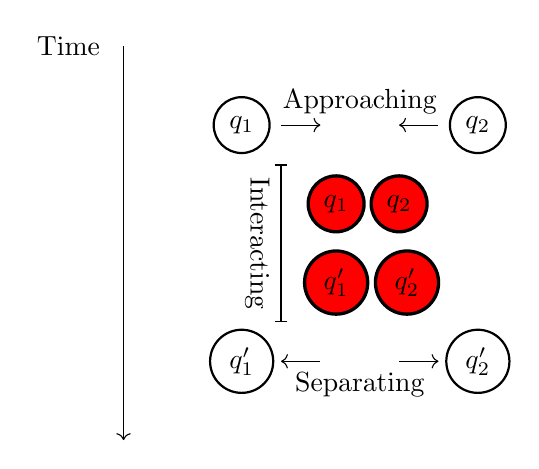
\begin{tikzpicture}
    [L0Node/.style={circle,   draw=black, thick, minimum size=7mm},
    L1Node/.style={circle,   draw=black, fill=red, very thick, minimum size=7mm}]
     \node[L0Node] (n0) at (0, 2){$q_1$};
     \node[L0Node] (n1) at (3, 2){$q_2$};
     \node[L1Node] (n2) at (1.2, 1){$q_1$};
     \node[L1Node] (n3) at (2.0, 1){$q_2$};
     \node[L1Node] (n4) at (1.2, 0){$q'_{1}$};
     \node[L1Node] (n5) at (2.1, 0){$q'_{2}$};
     \node[L0Node] (n6) at (0, -1){$q'_{1}$};
     \node[L0Node] (n7) at (3, -1){$q'_{2}$};
     \draw[->] (0.5,2) -- (1.0, 2);
     \draw[<-] (2,2) --  (2.5,2);
     \draw[<-] (0.5,-1) -- (1.0, -1);
     \draw[->] (2,-1) --  (2.5,-1);
     \draw[->] (-1.5,3) -- (-1.5, -2);
     \draw[|-|] (0.5,-0.5) -- (0.5,1.5);
     \node (TimeLabel) at (-2.2, 3){Time};
     \node (ApproachingLabel) at (1.5, 2.3){Approaching};
     \node (SeparatingLabel) at (1.5, -1.3){Separating};
     \node[rotate=-90]  (InteractingLabel) at (0.2, 0.5){Interacting};
\end{tikzpicture}
\end{center}
\caption{A typical (simple) interaction in population protocol}
\end{figure}



\par\noindent
The current implementation of this work assumes a more strict scheduler called random scheduler,
which resulting uniform random interactions (i.e. at each step, it presents
equally possibility for every pair of agents to interact.) Essentially, a random scheduler is a "fair" scheduler, but a "fair" scheduler is not necessarily a random scheduler.
The assumption actually increases the power of the model because it allows a leader agent detects the absence
of agents for a particular state after a long enough waiting \cite{AspnesR2007}. Note this is only for
simplifying the current implementation and possibly extends to other fair schedulers that is not a
random scheduler in the future.

\subsection{From Population Protocols to Network Constructor \cite{MS16a}}

\par\noindent
A variance of population protocol is called "network constructor" \cite{MS16a}.
It involves the extra elements do not existing in general population protocol called "edge", which is
the connection in between any two agents (or "processes") \cite{MS16a}. In general, the connection
is similar to the agents, on the characteristic that both of them have a finite number of states. For instance, if
a connection have $k + 1$ states,  state 0 may represent the connection does not exist and state $i \in \{1,2,3, ..., k\}$
show the strength for a particular connection.


\par\noindent
In the document and the currently implemented simulator, we solely consider the simplest
case containing only $on$ and $off$ two states for edges  \cite{MS16a}. A connection is said to be in
$on$ or $active$ state, if at any discrete time, the connection exists in between two
particular nodes; otherwise if the connection is stated as in $off$ or $inactive$ state  \cite{MS16a}.
At initial, all edge are in $off$ state, which means that there is no connection in a given
population at discrete time 0  \cite{MS16a}. The state for an edge may or may not change through an interaction
in between the two nodes that the edge currently connected or disconnected to.


\par\noindent
The network constructor also follows an adversary scheduler with "fairness" constraint. This is
exactly same as the paragraphs mentioned in the previous section \ref{IntroToPPFairScheduler}.

\paragraph{Formal Definition \cite{MS16a}}
Formally, a network constructor can be defined as:
\begin{itemize}
  \item $Q$, a finite set of passible states for an agent,
  \item $Q_{out}$, a finite set of output range,
  \item $q_{0} \in Q $, is initial state of node,
  \item $\delta: Q \times Q \times \{0,1\} \to Q \times Q \times \{0,1\}$, a transition function, where the $\{0,1\}$ is the states for edges with initial value 0.
\end{itemize}


\par\noindent
The main target of this model concentrates on network construction rather than
specific function computation, which is the task for general population protocol \cite{MS16a}. Notice that a transition can be either \textit{effective}
or \textit{ineffective}. Define $\delta(a, b, c) = (a^{'}, b^{'},c^{'})$ as a transition function (Here, $a, b$ are "node-state" whereas $c$ is state for edge.)
as it is in the formal definition, $\delta_{1}(a,b,c) = a^{'}$, $\delta_{2}(a,b,c) = b^{'}$ (representing two nodes states' change)
and $\delta_{3}(a,b,c) = c^{'}$ (representing edge state change), the transition $(a,b,c) \to (a^{'}, b^{'},c^{'})$ is called
effective if at least one $x \in \{a,b,c\} \not= x^{'} $; otherwise it is called ineffective \cite{MS16a}.


\par\noindent
Name the set of nodes (or "distributed processes" under this context) $V_{I}$ and the set of pairs of nodes as $E_{I}$.
A configuration $C$ is a mapping $ V_{I} \cup E_{I} \to Q \cup \{0,1\} $ determines the states of nodes and edges in the population at any discrete time.
The output of configuration $C$ is defined as the graph $G(C) = (V, E) $ where $V = \{u \in V_{I}: C(u) \in Q_{out}\}$
and  $E = \{uv: u, v \in V, u \not= v,$ and $C(uv) = 1\}$ \cite{MS16a}.



\subsection{Grid Terminating Network Constructor \cite{Mi17} \label{IntroToGrid}}

\par\noindent
Another paper \cite{Mi17} presents a different automata but very similar to network constructor. Each node in this
model has a fixed number of ports with it. In the 2-dimensional case, it will have 4 distinguished ports
$p_{y}$, $p_{x}$, $p_{-y}$ and $p_{-x}$, may simply donated as $u$, $r$, $d$ and $l$, respectively \cite{Mi17} .
The port, which neighbour with each other, are also perpendicular to each other, forming local axes. Hence,
$ u \perp r $, $ r \perp d $, $ d \perp l $, and  $ l \perp u $ \cite{Mi17} . The coordinates are only for local purposes and
do not necessarily represent the actual orientation of a node. A connection (or edge) can only be built through
pairs of ports, which is different from the previous model (network constructor).


\par\noindent
\begin{figure}[H]
\begin{center}
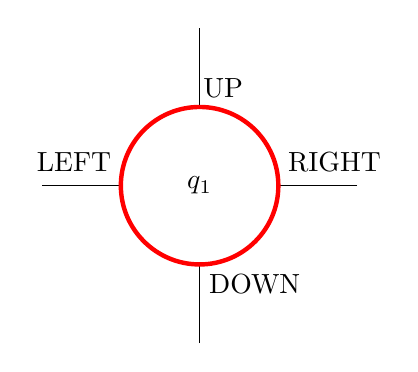
\begin{tikzpicture}
    \draw (2,0) -- (2,1);
    \draw (2,4) -- (2,3);
    \draw (0,2) -- (1,2);
    \draw (4,2) -- (3,2);
    \draw [red, ultra thick] (2,2) circle [radius=1];
    \node [below] at (2.7,1) {DOWN};
    \node [above] at (2.3,3) {UP};
    \node [left] at (1,2.3) {LEFT};
    \node [right] at (3,2.3) {RIGHT};
    \node [label] at (2,2) {$q_1$};
\end{tikzpicture}
\end{center}
\caption{Structure of a node in Grid Terminating Network Constructor model}
\end{figure}


\par\noindent
\paragraph{Formal Definition \cite{Mi17} }
Formally, a terminating grid network constructor in 2-D can be defined as:
\begin{itemize}
  \item $Q$, a finite set of passible states for an agent,
  \item $Q_{out}$, a finite set of output range,
  \item $q_{0} \in Q $, is initial state of node
  \item $\delta: (Q \times P ) \times (Q \times P) \times \{0,1\} \to Q \times Q \times \{0,1\}$, a transition function, where the $\{0,1\}$ is the states for edges with initial value 0.
  \item When required, there will be also a special initial leader-state $L_{0} \in Q $ defined.
\end{itemize}

\par\noindent
A transition can be either \textit{effective}
or \textit{ineffective}. Define $\delta((a, p_{1}), (b, p_{2}), c) = (a^{'}, b^{'},c^{'})$ as a transition function
as it is in the formal definition, it is called effective if at least one $x \in \{a,b,c\} \not= x^{'} $; otherwise it is called ineffective \cite{Mi17}.


\par\noindent
Every configuration $C$ forms a set of shapes $G[A(C)]$, where a shape means that the network induced
by active edges of $C$ \cite{Mi17}. Given the geometrical restrictions (i.e. the connection are
made at unit distance and are perpendicular whenever they correspond to consecutive ports of a node),
not all possible $A(C)$ are valid \cite{Mi17}. $A(C)$ is valid if any connected component defined by it is a
subnetwork of 2D grid network with the unit distance. A valid $A(C)$ at time $t -1$ also restricts the
possible valid $A(C)$ at time $t + k$, where $k \in Integer$ and $k \geq 0 $ \cite{Mi17}.


\par\noindent
The paper \cite{Mi17} also defines a set of
shapes $G_{out}(C) = \{V_{s}, E_{s}\}$ as output of a configuration where $V_{s} = \{u \in V : C_{v}(u) \in Q_{out} \}$
and $E_{s} = A(C) \cap \{ (v_{1}, p_{1}) : v_{1} \not= v_{2} \in V_{s}; p_{1}, p_{2} \in P \}$ \cite{Mi17}.
Less formally, the output shapes of a configuration contains all nodes in output states and the active edges in between them.
This model was designed as terminating protocols so it assumes $Q_{out} \subseteq Q_{halt} \subseteq Q $.
All rules containing $q_{halt} \in Q_{halt} $ is ineffective \cite{Mi17}.

\subsection{Existing solution}
There is an existing simulator called NETCS \cite{DBLP:journals/corr/AmaxilatisLMS15} for network constructor, which is the model covered
in this paper \cite{MS16a}. The simulator was written in Java, providing an web user interface
and assisting related research.

\par\noindent
This work will explore the possibility to simulate a further variance of network constructor, grid network constructor, as well as attempting
to provide a uniform simulation to different models and protocols, which would be easily extensible.

\subsection{Vector transformation: handle coordinate rotations in 2-dimension}


\par\noindent
As mentioned in the previous section \ref{IntroToGrid}, grid terminating network constructor enforces perpendicular ports
and geometrical restrictions. This means that handling rotation in some cases becomes necessary.
This section will cover some basic but related vector mathematics. The detailed algorithms will be discussed later on, in the section (\ref{design}).

\subsubsection{2D centred coordinate rotation, with origin point as the centre}

\par\noindent

\begin{figure}[H]
\begin{center}
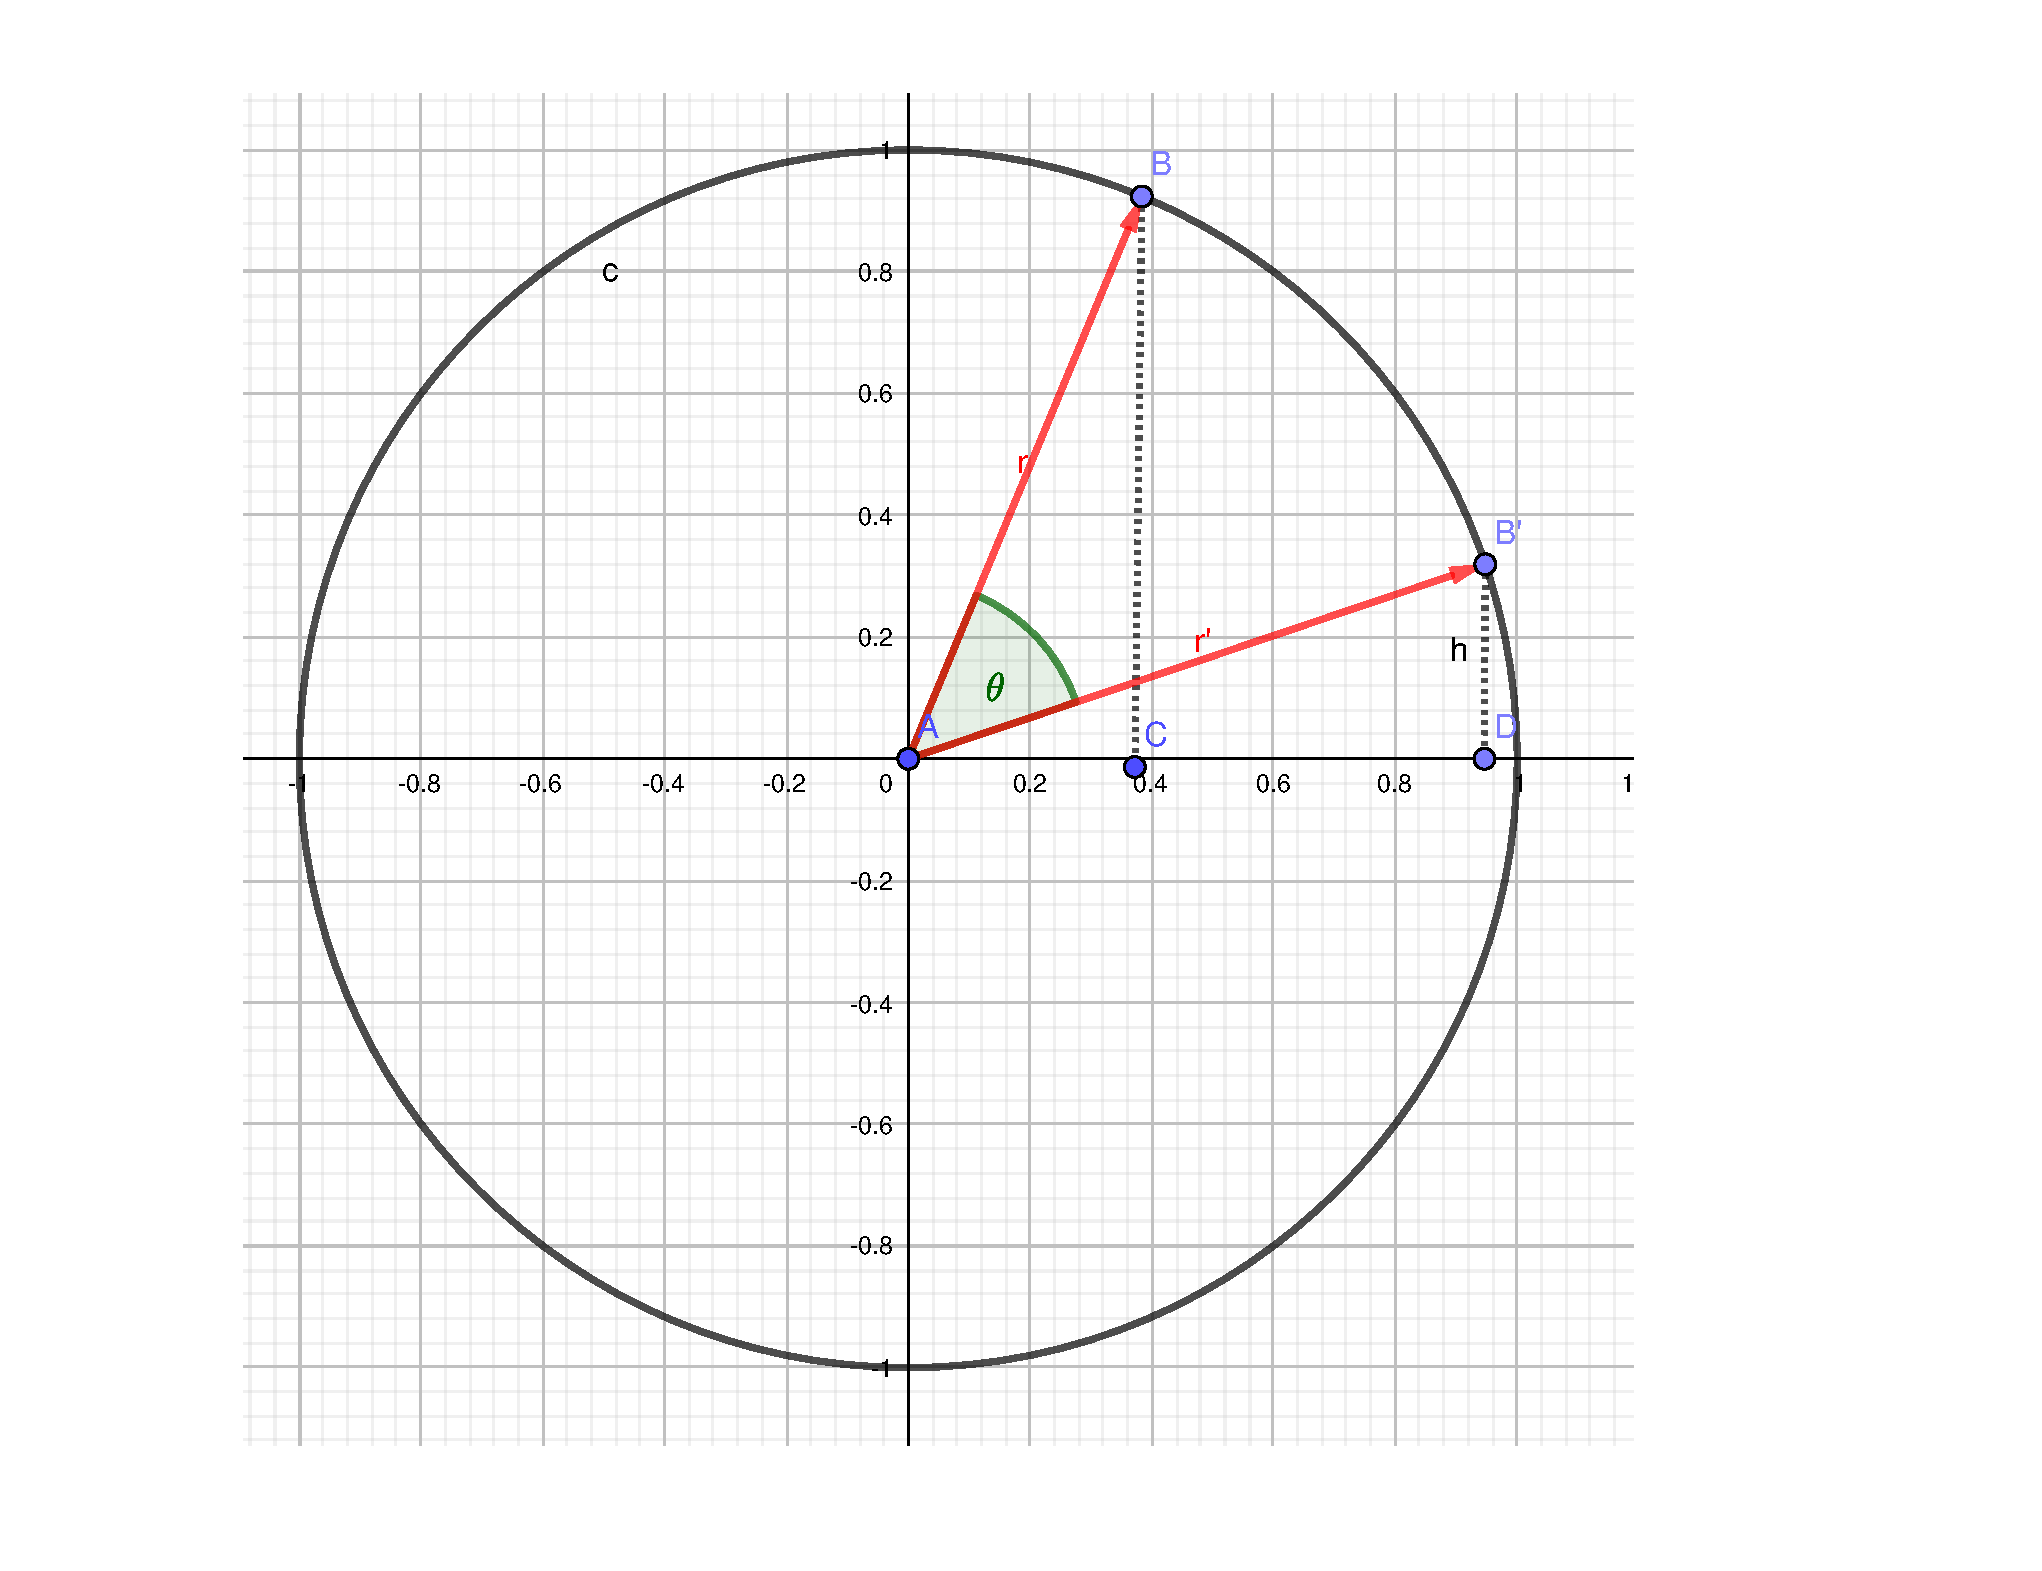
\includegraphics[width=0.5\textwidth]{context/diagram/2d_vector.pdf}
\caption{Vector $\vec{r}$ and $\vec{r_{'}}$ in unit circle}

\label{vectorG}
\end{center}
\end{figure}

\par\noindent
The figure \ref{vectorG} has two same-length vectors,  $\vec{r}$ (or $\vec{AB}$) and $\vec{r_{'}}$ (or $\vec{AB_{'}}$) in the Cartesian coordinate and their destination point located at the same unit circle.
The point $A$ is the origin point with coordinate $(0, 0)$. Suppose it has already known that the coordinate of $B$ is
$(x,y)$, and the $\theta$ angle. The question is that what the coordinate of $B^{'} $ (representing in $(x^{'},y^{'})$) is, after the first vector $\vec{r}$ rotating the given angle $\theta$ and becoming $\vec{r_{'}}$.
Note that, the "positive" rotation direction in current context and the implementation of the simulator is defined as "clock-wised".

\par\noindent
To solve this, the following equation can be concluded:

\begin{equation} \label{Equ_ori}
  \begin{bmatrix}
   x^{'} \\ y^{'}
   \end{bmatrix} =   \begin{bmatrix}
      \cos\theta & \sin\theta \\
      -\sin\theta & \cos\theta
    \end{bmatrix} \begin{bmatrix}
      x \\ y
     \end{bmatrix}
\end{equation}


\par\noindent
A brief derivation can be found in appendix below and it also can be found in \cite{Mitnote09} with a more precise and general proof.


\subsubsection{2D centred coordinate rotation, with any points as the centre}
Given the equation (\ref{Equ_ori}), it can be easily
deduced the fact that the rotation equation for any centred points $c$ with coordinate $(c_{x}, c_{y})$ can be achieved through
panning $c$ to origin point with coordinate $(0, 0)$, carry out the rotation and panning back to its original coordinate $(c_{x}, c_{y})$.
Suppose the target point that is required to be rotated is called $p$ (with coordinate $(x, y)$), it then has :
\begin{equation} \label{Equ_anycen}
  \begin{bmatrix}
   x^{'} \\ y^{'}
   \end{bmatrix} =   \begin{bmatrix}
      \cos\theta & \sin\theta \\
      -\sin\theta & \cos\theta
    \end{bmatrix} \left(\begin{bmatrix}
      x \\ y
     \end{bmatrix} - \begin{bmatrix}
       c_{x} \\ c_{y}
     \end{bmatrix}\right) + \begin{bmatrix}
        c_{x} \\ c_{y}
       \end{bmatrix}
\end{equation}
$p_{'}$ (with coordinate $(x_{'}, y_{'})$) will be point after $p$ rotating centred on $c$.
\subsubsection{Affine transformation form}
After a series of transformation, the equation \ref{Equ_anycen} becomes the following form:

\begin{equation} \label{Equ_aff}
  \begin{bmatrix}
   x^{'} \\ y^{'}
   \end{bmatrix}  = \begin{bmatrix} \cos\theta & \sin\theta \\ -\sin\theta & \cos\theta \end{bmatrix} \begin{bmatrix} x \\ y \end{bmatrix}
+ \begin{bmatrix} c_{x}(1 - \cos\theta) - c_{y}\sin\theta \\ c_{y}(1 - \cos\theta) + c_{x}\sin\theta \end{bmatrix}
\end{equation}

\par\noindent
Let $ \textbf{M} = \begin{bmatrix} \cos\theta & \sin\theta \\ -\sin\theta & \cos\theta \end{bmatrix} $
and $ \textbf{B} = \begin{bmatrix} c_{x}(1 - \cos\theta) - c_{y}\sin\theta \\ c_{y}(1 - \cos\theta) + c_{x}\sin\theta \end{bmatrix}$, then $ \begin{bmatrix} x^{'} \\ y^{'} \end{bmatrix}  = \textbf{M} \begin{bmatrix} x \\ y \end{bmatrix} + \textbf{B}$,
where it forms an \textit{affine transformation} \cite{WolframAT}. \textbf{M} and \textbf{B} can be calculated directly after knowing the rotation centre $(c_{x}, c_{y})$ and the
rotation agle $\theta$, and therefore the calculated \textbf{M} and  \textbf{B} can be applied for multiple target coordinates (those coordinates required to be rotated). This simplifies the calculation for a large batch of centred rotation with multiple target coordinates.




% \section {Data required} see website
% \section {Realisation \label{Realisation}} each stage & component; discuss problem encountered problem and solutions; testing (for each component); snapshot
% \section {Experiment  (optional)} propose; design of exp. ; exp. settings; discussion of results; chart and explain for chart
% \section {Evaluation} successful or not; how evaluate; who evaluate the project; strength and weakness of the project
% \section {Learning Points} [at least one page], story
% \section {Professional issues}  [at least one page] British Computer Society related to the project: Code of practice; Code of conduct
% \section Bio
% \section{Appendix} details of test data; (optional)more screen shot of sample; use guide; full design diagram
% zip of project

\section{Data Required}
There is also no real human data, real non-human data or human participants involved in the project.
For information used in papers, they are properly cited and referenced.
The simulator itself, developed based on some open sourced libraries, these
libraries are open to public and freely available in the public domain.
The list of open sources library and their licence would be listed as in appendix.

% \section {Design} <cross>copy & paste</cross> well modify & revise it; justify the changes
\section{Design}
\subsection{Anticipated components of the system}
\par\noindent
The main partition of the system was a software that enables to simulate
and visualise each interaction before convergence (or terminate). The project
would also attempt to explore one or more protocol to check their internal
status after finishing the software.

\par\noindent
The simulator would allow users to choose from a set of well-defined protocol and
specify the parameters for these protocol (e.g. number of agents participating).
The simulator would allow users to easily extend their own protocol though writing
structured few lines of code, an the extension should be as easy as possible.

\par\noindent
The system expected to have a ability to simulate some variations (which at
least includes the network constructor \cite{MS16a} and terminating grid network constructor in 2D \cite{Mi17})
of the original protocol according the protocol and dynamically visualise how process (nodes) transfer for each interaction.

\par\noindent
The interface provided would be a desktop application running on Java Virtual Machine Platform.
A web interface was desirable but would not be guaranteed to deliver.

\paragraph{Modification from original design}
\begin{itemize}
  \item The original design mentioned it could include "a configuration parser to
  enable user define a protocol from configuration files" finally replaced by a set of
  well-defined set of protocol and a programmable interface. This is because the
  original design requires a design and implementation of Domain Specific Language (DSL),
  and a parser of this kind of "new language", which is a large work load and might be
  infeasible to finish all of them
  during the project period. This might be done in the following development plan
  after finishing the project itself.
\end{itemize}

\subsection{Data structure, algorithms and Pseudo-code for key method}
\subsubsection{Adjacency List}
\par\noindent
For some specific kinds of models, specifically ,the network constructor, a data
structure to maintain a undirected graph $G$ formed from current configuration $C$ is required. In other words, it requires to maintain
a group of status of ”active” edges. It aims to construct ”shapes”
and there are some status for the edge $uv$ in between any nodes (processors) $u$
and $v$ in the population.

\par\noindent
To make it, an adjacency list would be used to record the connections associated
with each



\paragraph{Modification from original design}
\subsubsection{Graph}
\paragraph{Modification from original design}
\subsubsection{Terminating grid network constructor: Check acceptable configuration \& Handle rotation}  %mention BFS
\paragraph{Modification from original design}
\subsection{Interaction (Sequence) Design}
\begin{figure}[H]
\begin{center}
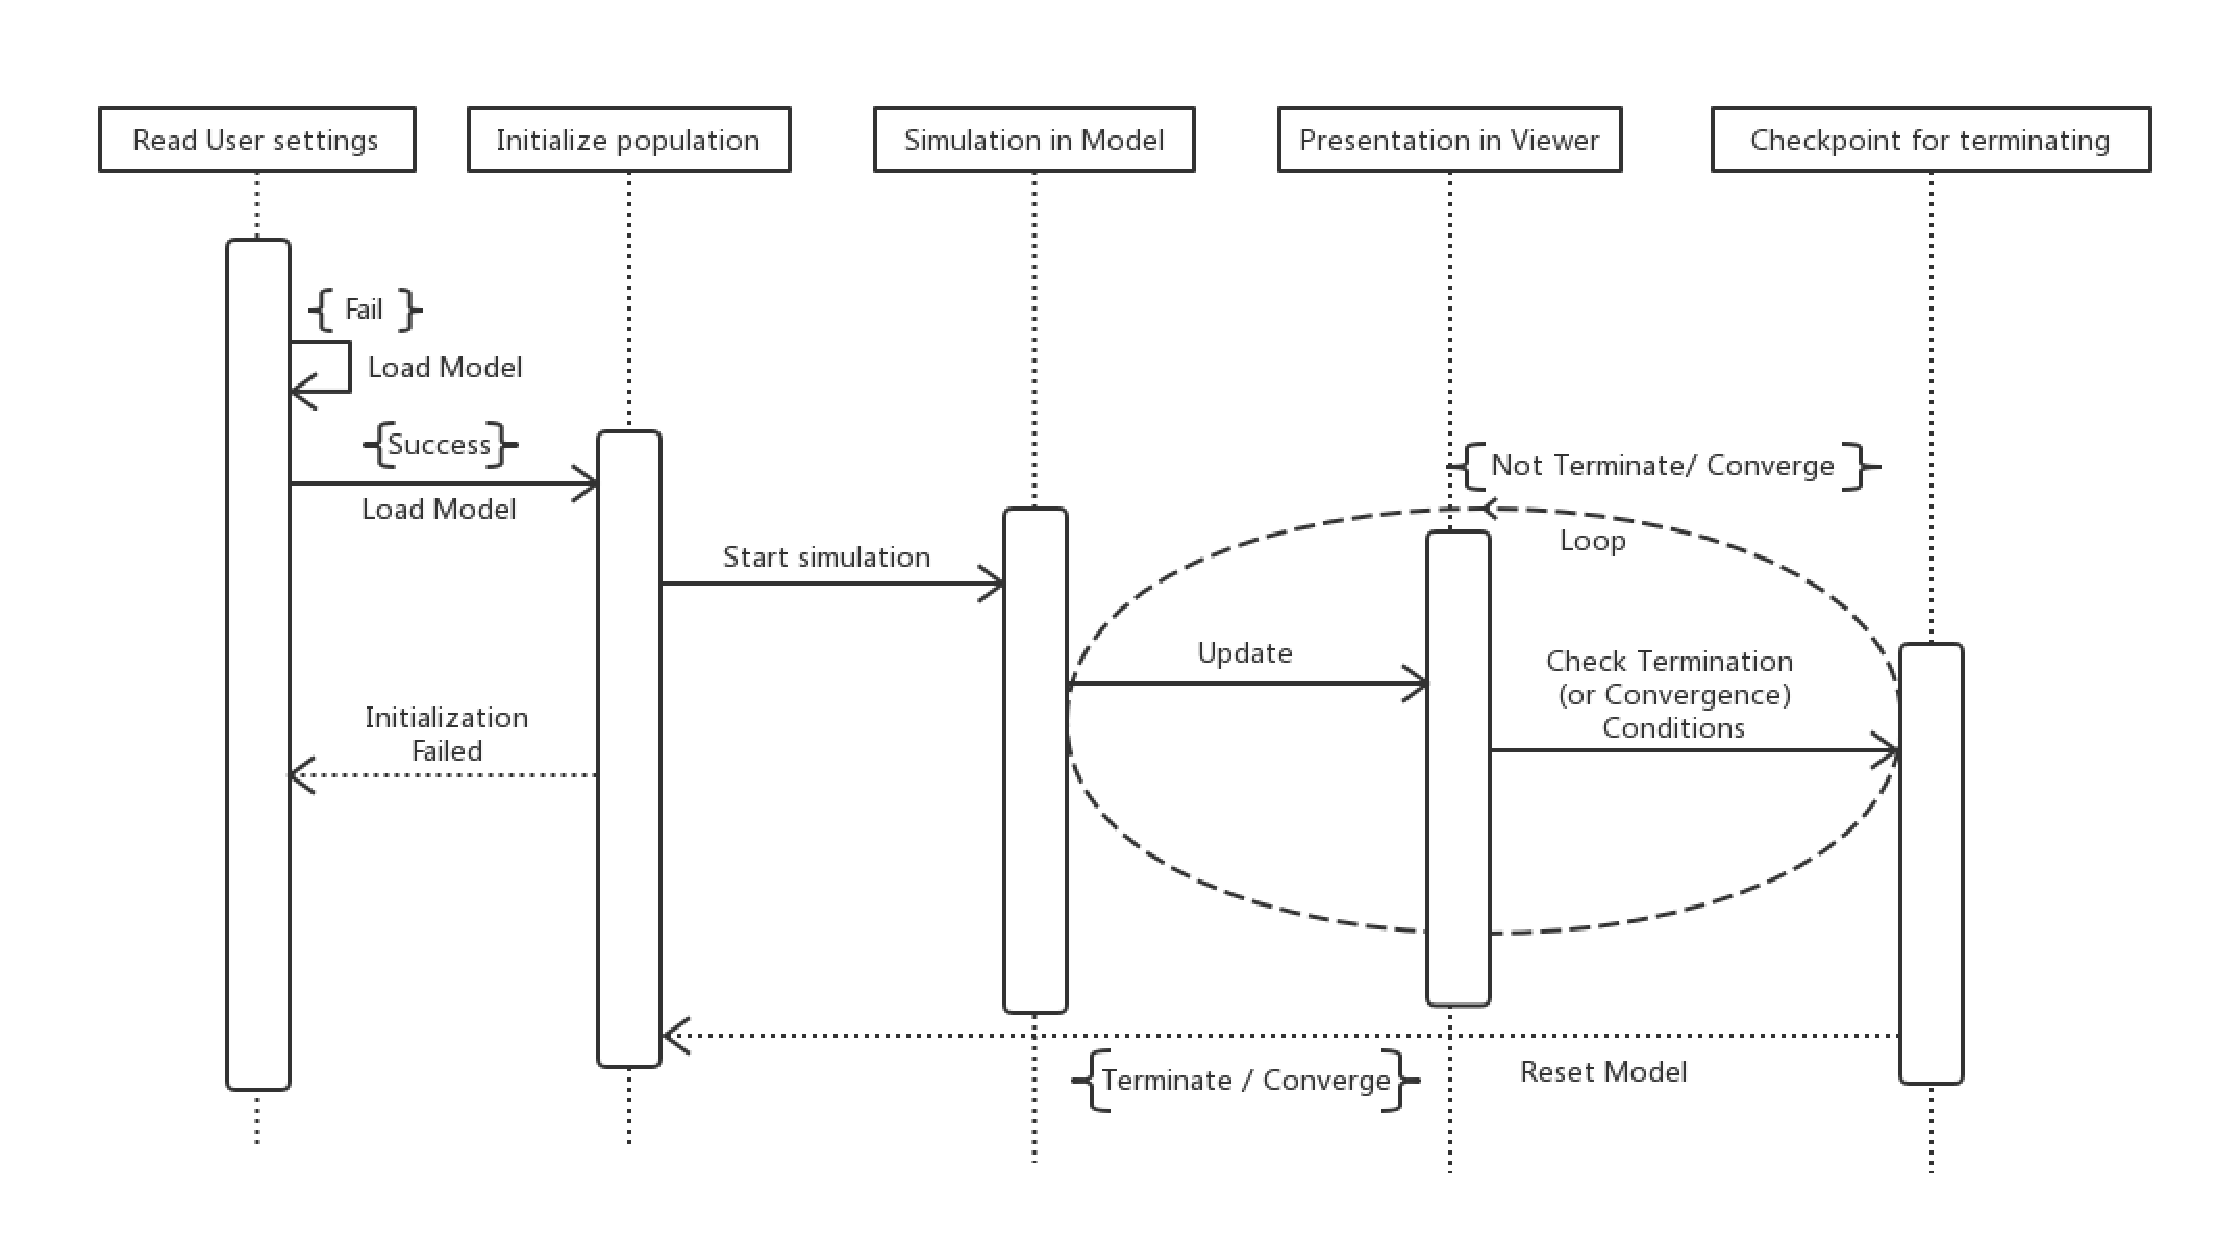
\includegraphics[width =\textwidth]{context/diagram/interaction.pdf}
\caption{Interaction Design Diagram}
\label{interactionG}
\end{center}
\end{figure}

\par\noindent
The figure \ref{interactionG} illustrates the entire interaction process of the
simulator. Initially, the user select one protocol from a set of well-defined
protocols and then select a set of parameters required such as how many nodes to
be included in the simulation, the initial status distribution for nodes and so forth.
Then the user click the "Apply settings button" to apply the model settings. before
applying the model, the program itself would check whether all parameters are
well-defined, i.e. locating in the value range they should be. If they are, the software
would load the model otherwise it will reject this particular request from user and
allow user to repeat its (possibly) another setting.

\par\noindent
After the program successfully loaded a model, the user can press the "Start simulation"
button to start a simulation. A simulation contains multiple rounds. For each round,
the model executes interaction simulation under the control of scheduler specified in one
of parameters mentioned before and then the model would update the states of elements
 in viewer to show the what happened in the model itself. Following that, the model would
 check whether it reaches a configuration that should stop the simulation. A stop can be caused
 by user's temporarily interruption (pause) or the fact that the number of consistent accumulation of
 inefficient interactions overwhelms a pre-configured parameters defined in the model (which indicates
 a terminating or convergence with a high possibility). If the model does not detect a stop,
 it will continue the "interact - update - checking stop" process as a loop. Once it detect a
 stop, the software will return to state of waiting for starting of a simulation process
 (while the model would keep its internal states and user can build an another new model under this situation).

 \paragraph{Modification from original design}
The current design removed a step of sequence in original sequence design called "Initialize scheduler", which located after "Initialize population" step.
the "Initialize scheduler" process had been integrated into "Initialize population" because
the scheduler partition does not necessarily separated from the population and can be treated as a partition of a "population" in concept.

\subsection{UI Interface Design}
\begin{figure}[H]
\begin{center}
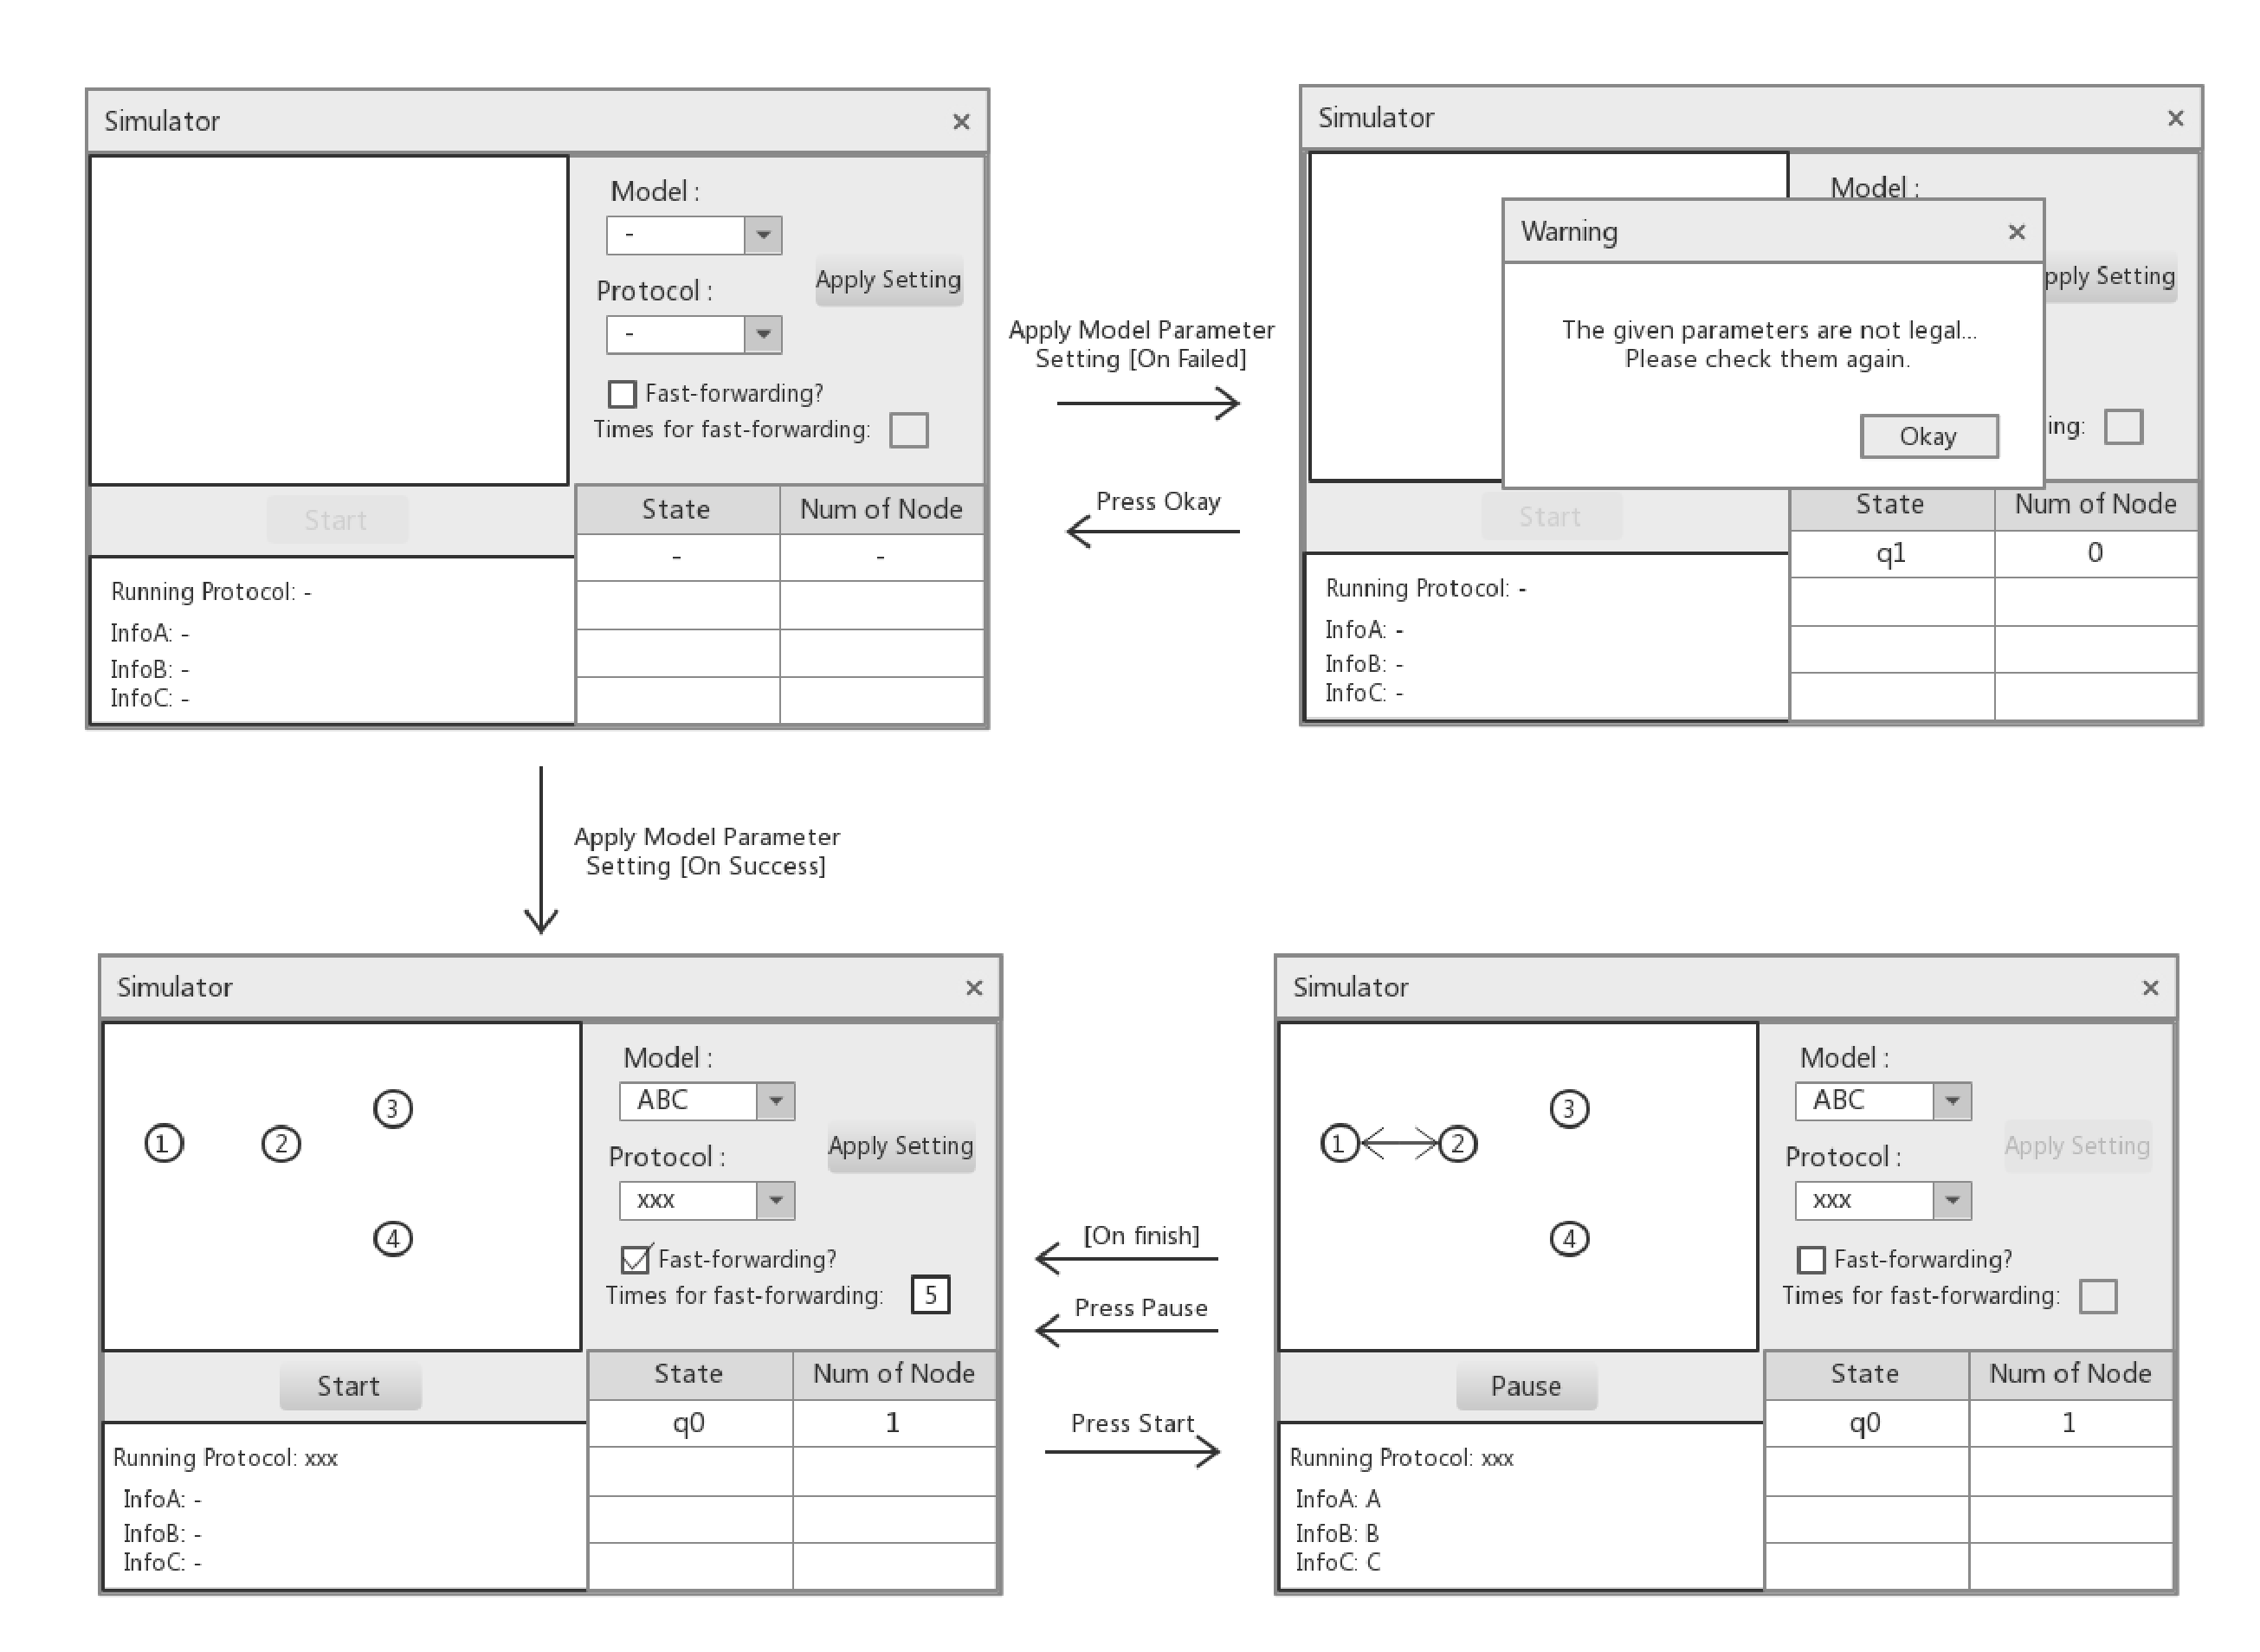
\includegraphics[width =\textwidth]{context/diagram/interface.pdf}
\caption{Interaction Design Diagram}
\label{intefaceG}
\end{center}
\end{figure}

\paragraph{Modification from original design}
The UI was redesigned entirely. This is because the original design built on the assumption
that the users load their settings for some population from domain specification language (DSL) codes residing in
some files. The DSL is infeasible to be finished due to the limited time of implementation.
Hence, the design would allow user to set their population through the UI containing a set of well-defined
protocols and would allow the users to write their own extensional protocol through few lines of codes.
As the functionality changes, the UI removed the functionality entrance for loading files from disk and
added some options to allow user setting the parameters of a protocol.

\section{Realisation}
\subsection{From Start of Realisation to 3rd March, 2018: implement first two models}
At very beginning, the first step was to attempt to implement the model of the
models including general population protocol \cite{AspnesR2007}, the network constructor \cite{MS16a} and
the terminating grid network constructor\cite{Mi17}. The first two is relatively easy because
they are much easier to be represented than the third one using widely used data structure
like adjacency list. For terminating grid network constructor, it is more complex in conception compared with
other two models. Hence it is failed to be done during this initial development period.
\paragraph{Construct software architecture}
During the development period, the most interfaces of model partition are finished according to the UML object
diagram mentioned in the \textit{design} section. An example could be the scheduler interface

\begin{lstlisting}[caption = {Interface design}, style = mykotlin]
//commit on Feb. 24th
interface Scheduler {
    fun select(population: Population): Pair<Node, Node>
}
\end{lstlisting}
\noindent
and grid network class without implementation.
\begin{lstlisting}[caption = {Grid network interface (early screenshot)}, style = mykotlin]
//commit on Feb. 24th
class NetworkConstructingPopulation constructor(scheduler: Scheduler) : LinkedPopulation {
    override val nodes: List<Node>
        get() = TODO("not implemented") //To change initializer of created properties use File | Settings | File Templates.

    override fun numOfEdge(): Int {
        TODO("not implemented") //To change body of created functions use File | Settings | File Templates.
    }

    override fun numOfNode(): Int {
        TODO("not implemented") //To change body of created functions use File | Settings | File Templates.
    }

    override fun interact(): Boolean {
        TODO("not implemented") //To change body of created functions use File | Settings | File Templates.
    }
\end{lstlisting}

\par\noindent
Though the method body not finished, these codes provides guidelines to the author for further development.
The language adopted in the project is Kotlin \cite{Kotlin}. This is A JVM language with support for pattern matching, high-order
function abstraction and operator overloading \cite{Kotlin}, which were essential characteristics for the development of this simulator.

\paragraph{Basic method for Handle centered rotation}
In the early stage, the author did aware that it would be necessary to handle centered rotation issues for terminating grid network model, hence
the author started to implement the rotation matrix, that is the equation \ref{Equ_ori}.

\begin{lstlisting}[caption = {Grid network interface (early screenshot)}, style = mykotlin]
import koma.end
import koma.extensions.get
import koma.extensions.map
import koma.mat
import koma.matrix.Matrix
import kotlin.math.roundToInt

//commit on Feb. 24th
data class LocallyCoordinatedNode(val x: Int,
                                  val y: Int,
                                  override val state: State, private val index: Int) : Node(state = state, index = index) {
    // IN-CLOCK direction rotation
    fun getLocallyRotatedNode(degree: Int): LocallyCoordinatedNode {
        val rad = degree * Math.PI / 180
        val transferMat = mat[
                Math.cos(rad), Math.sin(rad) end
                        0 - Math.sin(rad), Math.cos(rad)
                ]
        val transferred = (transferMat * mat[this.x, this.y].T).removeNegativeZeros()
        return LocallyCoordinatedNode(transferred[0, 0].roundToInt(), transferred[1, 0].roundToInt(), state, index)
    }

    private fun Matrix<Double>.removeNegativeZeros(): Matrix<Double> {
        return this.map { it -> if (it == -0.0) Math.abs(it) else it }
    }
}
\end{lstlisting}

\par\noindent
This is somehow a acceptable but naïve implementation for the only case that the rotation centre is the original point (0, 0)
and does not efficient for centred rotation involves multiple nodes needed to be rotated
(it might be optimised if taking the affine transformation form mentioned as in equation \ref{Equ_aff}).
The koma library , a scientific computing library written in Kotlin \cite{Koma}, is used here to simply the matrix calculation.
\par\noindent
Because in Kotlin, the $-0.0$ is defined as a different with $0.0$ for floating number and the value $-0.0$ is considered less than $0.0$ \cite{Kotlinfloat},
which causes issues in this calculation. Hence it is required to uniform the kind of different "$0$" using $removeNegativeZeros$ method.


\paragraph{Test-driven development}
At very first of beginning, the test codes for simple global line protocol (for testing network constructor model)
and dancing protocol (for testing general population protocol model) were written before any actual code is written. The test also included
a testing for node rotation (used later on for terminating grid network constructor). These test code written under JUnit framework \cite{JUnit}.

\par\noindent
Here is an example testing for rotation.
\begin{lstlisting}[caption = {Testing for rotation}, style = mykotlin]
//commit on Feb.24th
class LocallyCoordinatedNodeTest {

    @org.junit.Test
    fun rotationDegree() {
         // Create a node with locally coordinate (0, 0)
         val firstCase = LocallyCoordinatedNode(0, 0, State.createState(setOf("a", "b"), "a"), 1)
         // Make rotation
         val t90 = firstCase.getLocallyRotatedNode(90)
         val t180 = firstCase.getLocallyRotatedNode(180)
         val t270 = firstCase.getLocallyRotatedNode(270)
         val t360 = firstCase.getLocallyRotatedNode(360)

         assert(firstCase == t90)
         assert(firstCase == t180)
         assert(firstCase == t270)
         assert(firstCase == t360)
         // Create a node with locally coordinate (1, 1)
        `val secCase = LocallyCoordinatedNode(1, 1, State.createState(setOf("a", "b"), "a"), 1)
         //Make rotation
         val tt90 = secCase.getLocallyRotatedNode(90)
         val tt180 = secCase.getLocallyRotatedNode(180)
         val tt270 = secCase.getLocallyRotatedNode(270)
         val tt360 = secCase.getLocallyRotatedNode(360)
         assert(LocallyCoordinatedNode(1, -1, State.createState(setOf("a", "b"), "a"), 1) == tt90)
         assert(LocallyCoordinatedNode(-1, -1, State.createState(setOf("a", "b"), "a"), 1) == tt180)
         assert(LocallyCoordinatedNode(-1, 1, State.createState(setOf("a", "b"), "a"), 1) == tt270)
         assert(secCase == tt360)
    }

}
\end{lstlisting}

\subsection{From 3rd March to 26th March, 2018: Further progression}
\paragraph{Abstraction of interaction function \&\& implementation for some protocols}
During this stage, the three different interaction function concept appearing in the definition of the three models
were abstracted and represented using a Kotlin method (or say, a Kotlin function).
\begin{itemize}
  \item For general population protocol, it abstracted as
  \begin{lstlisting}[caption = {Abstraction for population protocol interaction function}, style = mykotlin]
      fun protocolFunc(initializer: ModelNode, receiver: ModelNode): Boolean
  \end{lstlisting}
   where the 1st and 2nd parameters are the two nodes selected to interact, the return value indicates whether the interaction happens ($true$ means it happens, $false$ means it not).
   \item For network constructor, it abstracted as
   \begin{lstlisting}[caption = {Abstraction for network constructor interaction function}, style = mykotlin]
      fun protocolFunc(initializer: ModelNode, receiver: ModelNode, adjacencyList: Map<ModelNode, HashSet<ModelNode>>): Pair<Boolean, Boolean>
   \end{lstlisting}
   where the 1st and 2nd parameters are the two nodes selected to interact, the 3rd parameter are the adjacency list (of which actual structure is a map) for the population that the
   first nodes located indicating the status of connection for the population. The first value in return pair indicates whether it is "effective" interaction
    (i.e. there is at least one changed state among 2 nodes and edge during the interaction, so $true$ means it is "effective", $false$ means not) while the
   second value in return pair indicates whether it is $active$ state for connection in between the two nodes after interaction($true$ means there it is active, $false$ means it is inactive).
   \item For terminating grid network, because the model is not well abstracted so it is not been abstracted successfully during this period.
\end{itemize}
\paragraph{Start of viewer implementation}
Consider the limited time for implementation, it reasonably considered as "infeasible" if building entire viewer system from sketch. The author used a dynamic
graph library called "GraphStream" \cite{GraphStream} to reduce the work amount to ensure a delivery on time.
GraphStream provides a set of basic tools for modelling dynamic graphs, such as representing elements of nodes and edges, which exactly suit for the scenario of the simulator.
\paragraph{Failed attempt to Domain Specific Language}
As initial design proposed, the author attempted to implement the functionality that allow user load their protocol from a file.
This involves loading a piece of user written code (in some Language) and then parse it into executable Kotlin code.
For time limited, it would be hard to implement a parser.
A few difficulties could be identified:
\begin{itemize}
  \item The computability of different models differs from each other. It is hard to be defined a standard set of calculation required to be supported.
  \item The form of language defined in papers requires further semantic interpretation to be transformed as executable code. A simple protocol
  sum (modulo 4) \cite{AspnesR2007} can illustrate this point. This protocol gathers the sum (modulo) of all agents to a single agent and the output
comes from the unique agent with a non-null value. The detailed rule of the protocol could be found in appendix.
Notice the rule $(v_{1}, v_{2}) \to (v_{1} + v_{2}, \bot_{v_{1} + v_{2}})$ involves an addition operation according to
the two inputs, an symbol substitution for one of output state (the second one) and a subscript addition for the second
output state. It would be a requirement to a set of powerful language grammar to define these operation if the language is required to express these operations.
\end{itemize}
A compromised but feasible solution is to utilise some language characteristics provided by Kotlin language such as operator overloading and infix expression \cite{Kotlin}.
Though defining some semantic meaning of some operations on the \textit{State} class, the transition function of sum (modulo 4) could be achieved.
Here is an implementation using this method.

\begin{lstlisting}[caption = {Implementation for transition function of sum (mod 4) protocol}, style = mykotlin]
fun sumModeFourFunc(initializer: ModelNode, receiver: ModelNode): Boolean {
    var isChanged = false
    val transferred = when{
        Pair(initializer.state,receiver.state) match Pair("[0123]","[0123]") ->{
            Pair((initializer.state + receiver.state)%4, "N" and ((initializer.state + receiver.state)%4))

        }
        Pair(initializer.state, receiver.state) match Pair("[0123]","N[0123]") -> {
            Pair(initializer.state,"N" and initializer.state)
        }

        else -> null
    }

    if (transferred!=null){
        initializer.state = transferred.first
        receiver.state = transferred.second
        isChanged = true
    }

    return isChanged
}\end{lstlisting}
\par\noindent
Note that in the implementation, there is some "new" keyword "match" and "and". The "match" keyword is used for regular expression matching,
where the first parameter before "match" keyword is the input state pair and the second parameter after this keyword is the pattern to be followed.
The "and" keyword concatenates a string and a state to produce proper results according to different situation.
\par\noindent
The \textit{initializer.state} and \textit{receiver.state} are instance of State.
The state class finally overrides (i.e. defines) 5 different binary operations including plus, minus, multiplication, division and module. The
defined operations can be modified or extended on request.

\subsection{From 27th March to 8th April, 2018: Implement terminating grid network constructor}
\paragraph{Model representation of terminating grid network constructor}
The model representation of grid network constructor has been covered in detail in the \textit{desgin} section. The
quad-direction linked structure was not initially proposed and was modified accordingly during this period of time.
The structure allow the model be modelled mathematically to follow geometrical restrictions
and limit the number of nodes connected to one nodes, which is also a limitation for this model.
\paragraph{View representation of terminating grid network constructor}
The basic concepts in the dynamic graph library, GraphStream \cite{GraphStream}, solely contains nodes, which may link to the "node (agent)" in
the three types of models to be simulated, and the edges, which may link to the "(active) connection between two nodes" for network simulator and
terminating grid network simulator. Nonetheless, there is no direct correspondence entity of "port" or "node with port" in the viewer library GraphStream.
It was required to define a node with "port" and specify what the outlook (or representation) of port.

\begin{figure}[H]
\begin{center}
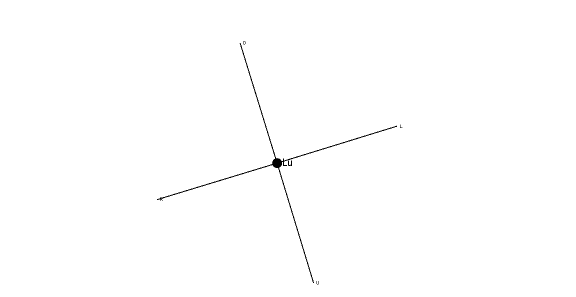
\includegraphics[width =0.7\textwidth]{context/diagram/GridNodeRepCapture.png}
\caption{Screenshot for a "node with port" in the viewer}
\label{capture_gridrep}
\end{center}
\end{figure}

\par\noindent
The figure \ref{capture_gridrep} is a typical representation of "a node with 4 ports" in terminating grid network constructor model. The centred node, which
is marked as $L_{u}$ is represented through a node representation in GraphStream. Here, to avoid any confusions, any elements including nodes and edges in
viewer part will be called as a representation while the nodes and edges in model part are still called its original name.
A port $p$ is actually another invisible node representation around the centred node $L_{u}$, and has visible line connected with $L_{u}$. Hence, a node
in terminating grid network constructor will be represented as a connected graph with 5 nodes and 4 edges in a star-like topology.

\par\noindent
Since the node representation is a graph in general, the basic manipulation of node representation in other will not suit for the node representation of
terminating grid network. Suppose there is a node representation has a real coordinate $(x_{np}, y_{np})$ (It is called "real coordinate" because the coordinate represents the true
location of the node representation and is distinct to the concept "relative coordinate" appearing in the model part.) and rotation degree $\theta_{np}$, and it intends to
another real coordinate $(x_{nq}, y_{nq})$, the movement would follows steps:
\begin{itemize}
  \item Move the centred node representation to coordinate $(x_{nq}, y_{nq})$
  \item Move the up port representation $p_{u}$ to coordinate to $(x_{nq}, y_{nq} + 1)$, right port $p_{r}$ representation to coordinate to $(x_{nq} + 1, y_{nq})$,  down port representation $p_{d}$ to coordinate to $(x_{nq}, y_{nq} - 1)$
  and left port $p_{l}$ representation to coordinate to $(x_{nq} - 1, y_{nq})$
  \item Do a centred rotation for $p_{u}$, $p_{l}$, $p_{r}$ ,$p_{d}$ regarding the centre $(x_{nq}, y_{nq})$ with rotation degree $\theta_{np}$
\end{itemize}
For rotation operation, after the centred node representation rotates, the 4 port representations are required to rotate the same degree that the centred node representation rotates.

\paragraph{Abstraction of interaction function of terminating grid network constructor}
After clarifying the model and view representation for the model, it finally could deduce the method signature for its transition function.
\begin{lstlisting}[caption = {Abstraction for terminating grid network constructor interaction function}, style = mykotlin]
  fun protocolFunc(
    firstPair: Pair<LocallyCoordinatedModelNode, Port>,
    secondPair: Pair<LocallyCoordinatedModelNode, Port>
    ): Triple<Boolean, Pair<String,String>, Boolean>
\end{lstlisting}
where the \textit{firstPair} refers the initializer node and port selected to interact and the \textit{secondPair} is the receiver.
There are three variables in the returned triple, where the first one indicates whether it is an effective interaction ($true$ if it is while $false$ for it is not), the second pair is the states
for the initializer node and receiver node respectively after the interaction, the third one indicates whether there is a "active" connection
in between two ports selected after the interaction ($true$ for there is while $false$ for there is not).

\subsection{From 9th April to 15th April, 2018: User Interface implementation and experiment}
\paragraph{Pause during simulation process and Fast-forward a simulation at initial}
The pausing function was implemented during the entire process but finishes during the final stage of implementation.
The viewer is following a "generator" pattern, which means its simulation is step based. At any time, it can stay in an intermediately
state and then resume at any time hence naturally results such a functionality.
\par\noindent
The fast-forwarding function allows user to specify a number for pre-executed selections (not number of interactions because some interactions may ineffective interactions),
and then show the results on the viewer directly after such that numbers of selections. This is normally fast then simulate in a step by step way. The key of this pattern is that
it simulates only in the model partition but does not demonstrate changes in the viewer part for initial steps, so this function will save a large amount of time from communication and synchronisation in between
model and viewer, and so from visualization animation.
\paragraph{Protocol expansibility}
Despite of the DSL was failed to be implemented, it was still possible to find some other ways to simply the process to define users' own protocols.
A possible solution might be reflection, which means “the ability of a program to manipulate as data something representing the state of the
program during its own execution" \cite{reflection96}.
\par\noindent
The simulator will check three particular classes with specific name
and check the functions and fields inside these classes that complies with some naming convention and load them if it possible when been launched each time.
More specifically, it has some classes called "protocol container", which of all implement \textit{InteractionFunctions} interface
and have their own companion object inside it. A well defined protocol $i$ contains three class static members with a same prefix, say $prefix_{i}$, in a protocol container.
The three class static members are named as "\textit{$prefix_{i}$InitialState}", "\textit{$prefix_{i}$Symbol}" and "\textit{$prefix_{i}$Func}", which are a map with String key and Int value defining the
initial configuration of the protocol, a set of String defining possible states that appearing in nodes and a function defines the transition function of a protocol.
\begin{itemize}
  \item For population protocol, the container is called \textit{PopulationProtocolFunctions}
  \item For network constructor, the container is called \textit{ShapeConstructionFunctions}
  \item For terminating grid network constructor, the container is called \textit{GridNetworkConstructingFunctions}
\end{itemize}
\par\noindent
The $prefix_{i}$ of a protocol $i$ is the "camel case" naming for the protocol and will be used in naming the protocol in user interface. For example,
a prefix "squareGridNetwork" will be presented as Square Grid Network in the simulator user interface.

\paragraph{Experiment to find ineffective protocols}
After finished the implementation of all main functionalities and built some protocols, the author examed some protocols to check their performance
and found that the dancing protocol may hard to converge under some settings. This is an evidence that the simulator is able dig into what happens inside
a protocol. A further details would be discussed later in \textit{evoluation} section.

\section{Learning Points}
This section will discussed some points that the author learned throughout the entire final year project process.
\subsection{Academic skills}
\paragraph{Basic understanding towards population protocols}
It was entirely an accidental for the author to select this topic as his final year project theme.
Dating back to one years' ago, the author saw the project description accidentally and find that it is possibly an attractive idea.
This is an area that few researchers focusing on compared with current research hotspot such as deep learning.
Though like that, the population protocol and network constructor provides a different perspective for what is computing and how computing works.

\paragraph{Applying mathematics into real project}
The research process involves some mathematics such as rotation matrix and trigonometric functions.
Though they are very basic, it is still a good practice to apply these knowledge learnt in book to solving the practical problems. It is truly
deepen the author's understanding towards linear algebra and trigonometric functions through working on this project.

\paragraph{Paper reading and information gathering}
Even for now, the author can only understand some partition of paper listed in bibliography but not all of them
because of his very limited knowledge, especially for some related mathematical knowledge, such as probability theory and
computational complexity theory.
However, this is also good train for the author to quick handle papers using his limited knowledge and to quick
gather useful information from related papers.

\paragraph{Academic writing and use of \LaTeX\ }
Though this is neither the first time that author write academic pieces nor first time
to use \LaTeX\ , this is still first time that the author using \LaTeX\ to finish a document that exceeds 20 pages.

\paragraph{Learning direction: Foundation knowledge}
The author found that he had some essential mathematic basics are not covered in his previous studies and
may start to his self-study in the near future.

\subsection{Technical (Development) skills}

\paragraph{Learnt a new language Kotlin and gained more understanding on programming language}
It was a proper choice for the author to take a risk for learning and using Kotlin rather than Java to finish
the project. Many language characteristics in Kotlin assisted the development process and simply the
implementation. The pattern matching, operator overloading and infix keyword deepen the author's understanding
towards programming language.

\paragraph{Had a better understanding on the relationship in between interface and model}
The application is all about how to cooperate the interface and model to enable them to work correctly and coherently.
Throughout the project, it took the author a large amount of time to construct the architecture of model and
user interface and to bridge them together.


\subsection{Soft skills}
\paragraph{Problem reduction and problem solving}
There were many problems that encountered in designed and development process finally
resolved through reducing problem to simpler case. For instance, the overlapping problem
for terminating grid network constructor could be resolved via discussion solution under
different situations. These solutions under different situations finally become the answer
to resolve the original problem.

\paragraph{Time management}
This entire development process teaches the author a lesson that practice
plan vitals. The author was failed to do so and led to a bad experience during
last period of development and dissertation writing.

\paragraph{Oral presentation}
The failure during requirement presentation enforced the author rethinking how to
properly deliver his context to his audience and optimise his strategy in his final
presentation through starting from easy concepts rather than presenting all core concepts at initial time of presentation.

\section{Professional issues}
The section will discuss how the project related to \textit{codes of conduct} \cite{bcsconduct} and \textit{codes of practice} \cite{bcspractic} issued by the British Computer Society (BCS).

\subsection{BCS codes of conduct \cite{bcsconduct}}
\paragraph{1. Public Interest}
The related software library \cite{Kotlin,Koma,GraphStream,JUnit} used is either licenced under Apache 2.0, or LGPLv3 or EPL 1.0, which all allow the
reference their software as the library in the code and these licenses are reasonably compatible with each other under the situation that the simulator only use them as a library and does not involve any modifications on them.
Any documents used in the document and in the associated application are well referenced. As clause \textbf{b} stated, "it have due regard for legitimate rights of third parties"\cite{bcsconduct}.

\par\noindent
There is no discrimination on any kind of basis during the entire process of development as the clause \textbf{c} stated.

\par\noindent
 The project had already opened its source code in https://github.com/billweasley/NetworkSimulator, so it could be considered as "promote equal access
 to benefits of IT as clause \textbf{d} stated".

\paragraph{2. Professional Competence and Integrity}
The entire document (this document) and software faithfully reflect my competence of understanding, which
follows what the clause \textbf{a, b} stated.

\paragraph{3. Duty to Relevant Authority}
The document and the entire project process is carefully in accordance with University of
Liverpool. There is no conflict of interest between the author and the University, which complies
with what the clause \textbf{a, b} stated.

\paragraph{4. Duty to Profession}
As mentioned before, the project would share its code online under LGPLv3 license and open to improvements, which by all means is
"encourage and support fellow members in their professional development" as clause \textbf{f} stated.

\subsection{BCS codes of practice \cite{bcspractic}}
\paragraph{When Defining a New Project and Planning}
The requirement document of the project "explained fully the deliverables"  and "ensures
the scope, deliverables, timescales, costs and responsibilities are agreed in advance" \cite{bcspractic}.
\par\noindent
A previous example "NETCS" \cite{DBLP:journals/corr/AmaxilatisLMS15} was found by the author and the author was inspired by its implementation.

\paragraph{When Tracking Progress}
The project was tracked using git commit history and it did not hide any overruns.

\paragraph{When Closing a Project}
As indicated in \cite{bcspractic}, the project summarise the mistakes made, good fortune encountered in \textit{Evaluation} section and
lessons learned in \textit{Learning points} section.
It also discussed further improvements that may benefits to this or other projects as suggested.

\clearpage
\makereference{reference.bib}
\clearpage
\appendix
\section{Brief Derivation for equation (\ref{Equ_ori})}
\par\noindent

For convenience, here name $\angle CAB $ as $\alpha$ in figure \ref{vectorG}. Then it has
$$|AD| = |\vec{r^{'}}| \cos(\alpha - \theta)$$
$$|B^{'}D| = |\vec{r^{'}}| \sin(\alpha - \theta)$$

By applying angle sum identities,
$$|AD| = |\vec{r^{'}}| (\cos(\alpha)\cos(-\theta) - \sin(\alpha)\sin(-\theta))$$
$$|B^{'}D| = |\vec{r^{'}}| (\sin(\alpha)\cos(-\theta) + \sin(-\theta)\cos(\alpha))$$

Because $|r^{'}| = |r|$, $\sin(\theta) = - \sin(-\theta)$ for $\theta \in [0, \pi/2)$ and $\cos(\theta) = \cos(-\theta)$ for $\theta \in [0, \pi/2)$,
$$|AD| = |\vec{r}| (\cos(\alpha)\cos(\theta) + \sin(\alpha)\sin(\theta))$$
$$|B^{'}D| = |\vec{r}| (\sin(\alpha)\cos(\theta) - \sin(\theta)\cos(\alpha))$$

Then,
$$|AD| = (|\vec{r}|\cos(\alpha))\cos(\theta) + (|\vec{r}|\sin(\alpha))\sin(\theta)$$
$$|B^{'}D| = (|\vec{r}|\sin(\alpha))\cos(\theta) - (|\vec{r}|\cos(\alpha))\sin(\theta)$$

Hence,
$$|AD| = |AC|\cos(\theta) + |BC|\sin(\theta)$$
$$|B^{'}D| = |BC|\cos(\theta) - |AC|\sin(\theta)$$

Finally,
$$|x^{'}| = |x|\cos(\theta) + |y|\sin(\theta)$$
$$|y^{'}| = |x|(- \sin(\theta)) + |y|\cos(\theta)$$

For $\theta \in [0, \pi/2)$, the equations can be written simply as
$$ x^{'} = x\cos\theta + y\sin\theta$$
$$ y^{'} = x(- \sin\theta) + y\cos\theta$$

which can be easily extended to $\theta \in [ 0, 2\pi + 2k\pi)$ via discussion under different cases, given that $k \in Integer$.\\

The two equations can be written in matrix form :
\begin{equation*}
  \begin{bmatrix}
   x^{'} \\ y^{'}
   \end{bmatrix} =   \begin{bmatrix}
      \cos\theta & \sin\theta \\
      -\sin\theta & \cos\theta
    \end{bmatrix} \begin{bmatrix}
      x \\ y
     \end{bmatrix}
\end{equation*}
\section{Brief Derivation for equation (\ref{Equ_aff})}
\par\noindent
The equation \ref{Equ_anycen} can be transformed to:
\begin{equation*}
  \begin{split}
  \begin{bmatrix}
   x^{'} \\ y^{'}
   \end{bmatrix} &= \begin{bmatrix} \cos\theta & \sin\theta \\ -\sin\theta & \cos\theta \end{bmatrix} \left(\begin{bmatrix} x \\ y \end{bmatrix} - \begin{bmatrix} c_{x} \\ c_{y} \end{bmatrix}\right) + \begin{bmatrix} c_{x} \\ c_{y} \end{bmatrix} \\
                 &= \begin{bmatrix}
          \cos\theta & \sin\theta \\
          -\sin\theta & \cos\theta
        \end{bmatrix}
        \begin{bmatrix}
          x \\ y
         \end{bmatrix} - \begin{bmatrix}
            \cos\theta & \sin\theta \\
            -\sin\theta & \cos\theta
          \end{bmatrix}\begin{bmatrix}
            c_{x} \\ c_{y}
          \end{bmatrix} + \begin{bmatrix}
            c_{x} \\ c_{y}
          \end{bmatrix} \\
          &= \begin{bmatrix} \cos\theta & \sin\theta \\ -\sin\theta & \cos\theta \end{bmatrix} \begin{bmatrix} x \\ y \end{bmatrix}
          - \begin{bmatrix} c_{x}\cos\theta + c_{y}\sin\theta \\ -c_{x}\sin\theta + c_{y}\cos\theta \end{bmatrix} +
           \begin{bmatrix} c_{x} \\ c_{y} \end{bmatrix} \\
          &= \begin{bmatrix} \cos\theta & \sin\theta \\ -\sin\theta & \cos\theta \end{bmatrix} \begin{bmatrix} x \\ y \end{bmatrix}
          + \begin{bmatrix} c_{x}(1 - \cos\theta) - c_{y}\sin\theta \\ c_{y}(1 - \cos\theta) + c_{x}\sin\theta \end{bmatrix}
\end{split}
\end{equation*}

\end{document}
